\documentclass{standalone}
\usepackage{tikz}
\usetikzlibrary{decorations.pathmorphing,arrows.meta}

\begin{document}
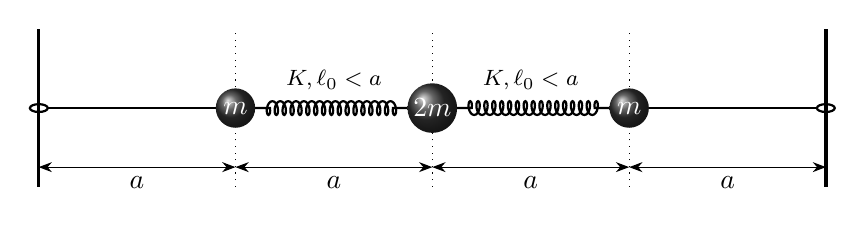
\begin{tikzpicture}
\coordinate (A) at (-2.5,0);
\coordinate (B) at (0,0);
\coordinate (C) at (2.5,0);

\draw[very thick](-5,-1)--(-5,1);
\draw[very thick](5,-1)--(5,1);

\draw[thick,decoration={coil,aspect=-.5,post length=0.35cm,segment length=1mm,pre length=0.5cm},decorate](B)--node[yshift=10]{\footnotesize $K,\ell_0<a$}(A);
\draw[thick,decoration={coil,aspect=-.5,post length=0.35cm,segment length=1mm,pre length=0.5cm},decorate](B)--node[yshift=10]{\footnotesize $K,\ell_0<a$}(C);
\draw[thick,{Ellipse[open]}-](-5.125,0|-A)--(A);
\draw[thick,{Ellipse[open]}-](5.125,0|-C)--(C);

\foreach \x in {-2.5,0,2.5} \draw[dotted](\x,-1)--(\x,1);

\shade[ball color=black!80](A)circle(0.25)node[]{\color{white} $m$};
\shade[ball color=black!80](B)circle(0.315)node[]{\color{white} $2m$};
\shade[ball color=black!80](C)circle(0.25)node[]{\color{white} $m$};

\draw[{Stealth[]}-{Stealth[]}](-5,-0.75)--node[anchor=north]{$a$}(-2.5,-0.75);
\draw[{Stealth[]}-{Stealth[]}](-2.5,-0.75)--node[anchor=north]{$a$}(0,-0.75);
\draw[{Stealth[]}-{Stealth[]}](0,-0.75)--node[anchor=north]{$a$}(2.5,-0.75);
\draw[{Stealth[]}-{Stealth[]}](2.5,-0.75)--node[anchor=north]{$a$}(5,-0.75);

\end{tikzpicture}
\end{document}